% Created by tikzDevice version 0.10.1 on 2018-01-25 16:21:31
% !TEX encoding = UTF-8 Unicode
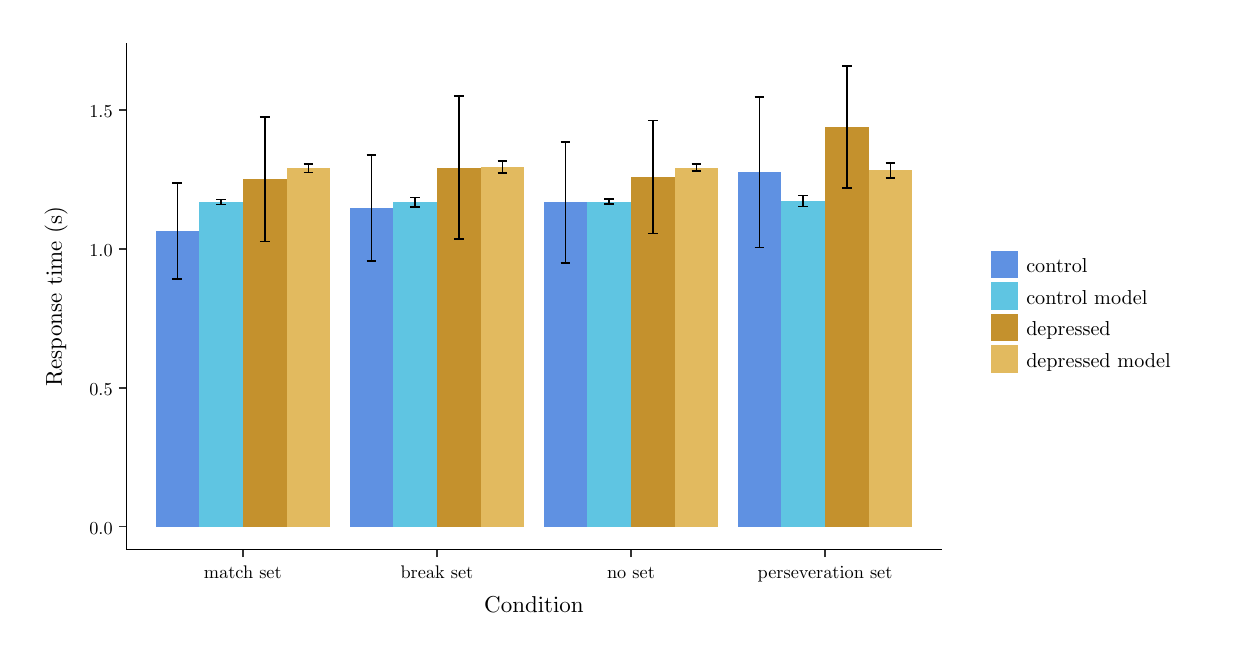
\begin{tikzpicture}[x=1pt,y=1pt]
\definecolor{fillColor}{RGB}{255,255,255}
\path[use as bounding box,fill=fillColor,fill opacity=0.00] (0,0) rectangle (433.62,216.81);
\begin{scope}
\path[clip] (  0.00,  0.00) rectangle (433.62,216.81);
\definecolor{drawColor}{RGB}{255,255,255}
\definecolor{fillColor}{RGB}{255,255,255}

\path[draw=drawColor,line width= 0.6pt,line join=round,line cap=round,fill=fillColor] (  0.00,  0.00) rectangle (433.62,216.81);
\end{scope}
\begin{scope}
\path[clip] ( 35.67, 28.22) rectangle (330.22,211.31);
\definecolor{fillColor}{RGB}{255,255,255}

\path[fill=fillColor] ( 35.67, 28.22) rectangle (330.22,211.31);
\definecolor{fillColor}{RGB}{226,186,95}

\path[fill=fillColor] ( 93.53, 36.55) rectangle (109.31,165.99);
\definecolor{fillColor}{RGB}{196,145,45}

\path[fill=fillColor] ( 77.75, 36.55) rectangle ( 93.53,161.98);
\definecolor{fillColor}{RGB}{95,197,226}

\path[fill=fillColor] ( 61.97, 36.55) rectangle ( 77.75,153.83);
\definecolor{fillColor}{RGB}{95,145,226}

\path[fill=fillColor] ( 46.19, 36.55) rectangle ( 61.97,143.31);
\definecolor{fillColor}{RGB}{226,186,95}

\path[fill=fillColor] (163.66, 36.55) rectangle (179.44,166.45);
\definecolor{fillColor}{RGB}{196,145,45}

\path[fill=fillColor] (147.88, 36.55) rectangle (163.66,166.19);
\definecolor{fillColor}{RGB}{95,197,226}

\path[fill=fillColor] (132.10, 36.55) rectangle (147.88,153.71);
\definecolor{fillColor}{RGB}{95,145,226}

\path[fill=fillColor] (116.32, 36.55) rectangle (132.10,151.61);
\definecolor{fillColor}{RGB}{226,186,95}

\path[fill=fillColor] (233.79, 36.55) rectangle (249.57,166.26);
\definecolor{fillColor}{RGB}{196,145,45}

\path[fill=fillColor] (218.01, 36.55) rectangle (233.79,162.82);
\definecolor{fillColor}{RGB}{95,197,226}

\path[fill=fillColor] (202.23, 36.55) rectangle (218.01,153.93);
\definecolor{fillColor}{RGB}{95,145,226}

\path[fill=fillColor] (186.45, 36.55) rectangle (202.23,153.68);
\definecolor{fillColor}{RGB}{226,186,95}

\path[fill=fillColor] (303.92, 36.55) rectangle (319.70,165.25);
\definecolor{fillColor}{RGB}{196,145,45}

\path[fill=fillColor] (288.14, 36.55) rectangle (303.92,180.98);
\definecolor{fillColor}{RGB}{95,197,226}

\path[fill=fillColor] (272.36, 36.55) rectangle (288.14,154.14);
\definecolor{fillColor}{RGB}{95,145,226}

\path[fill=fillColor] (256.58, 36.55) rectangle (272.36,164.55);
\definecolor{drawColor}{RGB}{0,0,0}

\path[draw=drawColor,line width= 0.6pt,line join=round] ( 99.67,167.49) --
	(103.17,167.49);

\path[draw=drawColor,line width= 0.6pt,line join=round] (101.42,167.49) --
	(101.42,164.48);

\path[draw=drawColor,line width= 0.6pt,line join=round] ( 99.67,164.48) --
	(103.17,164.48);

\path[draw=drawColor,line width= 0.6pt,line join=round] ( 83.89,184.46) --
	( 87.39,184.46);

\path[draw=drawColor,line width= 0.6pt,line join=round] ( 85.64,184.46) --
	( 85.64,139.50);

\path[draw=drawColor,line width= 0.6pt,line join=round] ( 83.89,139.50) --
	( 87.39,139.50);

\path[draw=drawColor,line width= 0.6pt,line join=round] ( 68.11,154.71) --
	( 71.62,154.71);

\path[draw=drawColor,line width= 0.6pt,line join=round] ( 69.86,154.71) --
	( 69.86,152.95);

\path[draw=drawColor,line width= 0.6pt,line join=round] ( 68.11,152.95) --
	( 71.62,152.95);

\path[draw=drawColor,line width= 0.6pt,line join=round] ( 52.33,160.71) --
	( 55.84,160.71);

\path[draw=drawColor,line width= 0.6pt,line join=round] ( 54.08,160.71) --
	( 54.08,125.92);

\path[draw=drawColor,line width= 0.6pt,line join=round] ( 52.33,125.92) --
	( 55.84,125.92);

\path[draw=drawColor,line width= 0.6pt,line join=round] (169.80,168.73) --
	(173.30,168.73);

\path[draw=drawColor,line width= 0.6pt,line join=round] (171.55,168.73) --
	(171.55,164.18);

\path[draw=drawColor,line width= 0.6pt,line join=round] (169.80,164.18) --
	(173.30,164.18);

\path[draw=drawColor,line width= 0.6pt,line join=round] (154.02,192.05) --
	(157.52,192.05);

\path[draw=drawColor,line width= 0.6pt,line join=round] (155.77,192.05) --
	(155.77,140.34);

\path[draw=drawColor,line width= 0.6pt,line join=round] (154.02,140.34) --
	(157.52,140.34);

\path[draw=drawColor,line width= 0.6pt,line join=round] (138.24,155.41) --
	(141.74,155.41);

\path[draw=drawColor,line width= 0.6pt,line join=round] (139.99,155.41) --
	(139.99,152.01);

\path[draw=drawColor,line width= 0.6pt,line join=round] (138.24,152.01) --
	(141.74,152.01);

\path[draw=drawColor,line width= 0.6pt,line join=round] (122.46,170.84) --
	(125.97,170.84);

\path[draw=drawColor,line width= 0.6pt,line join=round] (124.21,170.84) --
	(124.21,132.38);

\path[draw=drawColor,line width= 0.6pt,line join=round] (122.46,132.38) --
	(125.97,132.38);

\path[draw=drawColor,line width= 0.6pt,line join=round] (239.93,167.54) --
	(243.43,167.54);

\path[draw=drawColor,line width= 0.6pt,line join=round] (241.68,167.54) --
	(241.68,164.98);

\path[draw=drawColor,line width= 0.6pt,line join=round] (239.93,164.98) --
	(243.43,164.98);

\path[draw=drawColor,line width= 0.6pt,line join=round] (224.15,183.25) --
	(227.65,183.25);

\path[draw=drawColor,line width= 0.6pt,line join=round] (225.90,183.25) --
	(225.90,142.38);

\path[draw=drawColor,line width= 0.6pt,line join=round] (224.15,142.38) --
	(227.65,142.38);

\path[draw=drawColor,line width= 0.6pt,line join=round] (208.37,154.81) --
	(211.87,154.81);

\path[draw=drawColor,line width= 0.6pt,line join=round] (210.12,154.81) --
	(210.12,153.05);

\path[draw=drawColor,line width= 0.6pt,line join=round] (208.37,153.05) --
	(211.87,153.05);

\path[draw=drawColor,line width= 0.6pt,line join=round] (192.59,175.56) --
	(196.09,175.56);

\path[draw=drawColor,line width= 0.6pt,line join=round] (194.34,175.56) --
	(194.34,131.81);

\path[draw=drawColor,line width= 0.6pt,line join=round] (192.59,131.81) --
	(196.09,131.81);

\path[draw=drawColor,line width= 0.6pt,line join=round] (310.05,167.93) --
	(313.56,167.93);

\path[draw=drawColor,line width= 0.6pt,line join=round] (311.81,167.93) --
	(311.81,162.57);

\path[draw=drawColor,line width= 0.6pt,line join=round] (310.05,162.57) --
	(313.56,162.57);

\path[draw=drawColor,line width= 0.6pt,line join=round] (294.28,202.99) --
	(297.78,202.99);

\path[draw=drawColor,line width= 0.6pt,line join=round] (296.03,202.99) --
	(296.03,158.97);

\path[draw=drawColor,line width= 0.6pt,line join=round] (294.28,158.97) --
	(297.78,158.97);

\path[draw=drawColor,line width= 0.6pt,line join=round] (278.50,156.12) --
	(282.00,156.12);

\path[draw=drawColor,line width= 0.6pt,line join=round] (280.25,156.12) --
	(280.25,152.16);

\path[draw=drawColor,line width= 0.6pt,line join=round] (278.50,152.16) --
	(282.00,152.16);

\path[draw=drawColor,line width= 0.6pt,line join=round] (262.72,191.78) --
	(266.22,191.78);

\path[draw=drawColor,line width= 0.6pt,line join=round] (264.47,191.78) --
	(264.47,137.33);

\path[draw=drawColor,line width= 0.6pt,line join=round] (262.72,137.33) --
	(266.22,137.33);
\end{scope}
\begin{scope}
\path[clip] (  0.00,  0.00) rectangle (433.62,216.81);
\definecolor{drawColor}{RGB}{0,0,0}

\path[draw=drawColor,line width= 0.6pt,line join=round] ( 35.67, 28.22) --
	( 35.67,211.31);
\end{scope}
\begin{scope}
\path[clip] (  0.00,  0.00) rectangle (433.62,216.81);
\definecolor{drawColor}{RGB}{0,0,0}

\node[text=drawColor,anchor=base east,inner sep=0pt, outer sep=0pt, scale=  0.66] at ( 30.72, 33.82) {0.0};

\node[text=drawColor,anchor=base east,inner sep=0pt, outer sep=0pt, scale=  0.66] at ( 30.72, 83.99) {0.5};

\node[text=drawColor,anchor=base east,inner sep=0pt, outer sep=0pt, scale=  0.66] at ( 30.72,134.17) {1.0};

\node[text=drawColor,anchor=base east,inner sep=0pt, outer sep=0pt, scale=  0.66] at ( 30.72,184.34) {1.5};
\end{scope}
\begin{scope}
\path[clip] (  0.00,  0.00) rectangle (433.62,216.81);
\definecolor{drawColor}{gray}{0.20}

\path[draw=drawColor,line width= 0.6pt,line join=round] ( 32.92, 36.55) --
	( 35.67, 36.55);

\path[draw=drawColor,line width= 0.6pt,line join=round] ( 32.92, 86.72) --
	( 35.67, 86.72);

\path[draw=drawColor,line width= 0.6pt,line join=round] ( 32.92,136.89) --
	( 35.67,136.89);

\path[draw=drawColor,line width= 0.6pt,line join=round] ( 32.92,187.07) --
	( 35.67,187.07);
\end{scope}
\begin{scope}
\path[clip] (  0.00,  0.00) rectangle (433.62,216.81);
\definecolor{drawColor}{RGB}{0,0,0}

\path[draw=drawColor,line width= 0.6pt,line join=round] ( 35.67, 28.22) --
	(330.22, 28.22);
\end{scope}
\begin{scope}
\path[clip] (  0.00,  0.00) rectangle (433.62,216.81);
\definecolor{drawColor}{gray}{0.20}

\path[draw=drawColor,line width= 0.6pt,line join=round] ( 77.75, 25.47) --
	( 77.75, 28.22);

\path[draw=drawColor,line width= 0.6pt,line join=round] (147.88, 25.47) --
	(147.88, 28.22);

\path[draw=drawColor,line width= 0.6pt,line join=round] (218.01, 25.47) --
	(218.01, 28.22);

\path[draw=drawColor,line width= 0.6pt,line join=round] (288.14, 25.47) --
	(288.14, 28.22);
\end{scope}
\begin{scope}
\path[clip] (  0.00,  0.00) rectangle (433.62,216.81);
\definecolor{drawColor}{RGB}{0,0,0}

\node[text=drawColor,anchor=base,inner sep=0pt, outer sep=0pt, scale=  0.66] at ( 77.75, 17.82) {match set};

\node[text=drawColor,anchor=base,inner sep=0pt, outer sep=0pt, scale=  0.66] at (147.88, 17.82) {break set};

\node[text=drawColor,anchor=base,inner sep=0pt, outer sep=0pt, scale=  0.66] at (218.01, 17.82) {no set};

\node[text=drawColor,anchor=base,inner sep=0pt, outer sep=0pt, scale=  0.66] at (288.14, 17.82) {perseveration set};
\end{scope}
\begin{scope}
\path[clip] (  0.00,  0.00) rectangle (433.62,216.81);
\definecolor{drawColor}{RGB}{0,0,0}

\node[text=drawColor,anchor=base,inner sep=0pt, outer sep=0pt, scale=  0.83] at (182.95,  5.50) {Condition};
\end{scope}
\begin{scope}
\path[clip] (  0.00,  0.00) rectangle (433.62,216.81);
\definecolor{drawColor}{RGB}{0,0,0}

\node[text=drawColor,rotate= 90.00,anchor=base,inner sep=0pt, outer sep=0pt, scale=  0.83] at ( 12.32,119.77) {Response time (s)};
\end{scope}
\begin{scope}
\path[clip] (  0.00,  0.00) rectangle (433.62,216.81);
\definecolor{fillColor}{RGB}{255,255,255}

\path[fill=fillColor] (341.60, 85.74) rectangle (428.12,153.80);
\end{scope}
\begin{scope}
\path[clip] (  0.00,  0.00) rectangle (433.62,216.81);
\definecolor{fillColor}{RGB}{95,145,226}

\path[fill=fillColor] (348.00,126.28) rectangle (357.96,136.24);
\end{scope}
\begin{scope}
\path[clip] (  0.00,  0.00) rectangle (433.62,216.81);
\definecolor{fillColor}{RGB}{95,197,226}

\path[fill=fillColor] (348.00,114.90) rectangle (357.96,124.86);
\end{scope}
\begin{scope}
\path[clip] (  0.00,  0.00) rectangle (433.62,216.81);
\definecolor{fillColor}{RGB}{196,145,45}

\path[fill=fillColor] (348.00,103.52) rectangle (357.96,113.48);
\end{scope}
\begin{scope}
\path[clip] (  0.00,  0.00) rectangle (433.62,216.81);
\definecolor{fillColor}{RGB}{226,186,95}

\path[fill=fillColor] (348.00, 92.14) rectangle (357.96,102.10);
\end{scope}
\begin{scope}
\path[clip] (  0.00,  0.00) rectangle (433.62,216.81);
\definecolor{drawColor}{RGB}{0,0,0}

\node[text=drawColor,anchor=base west,inner sep=0pt, outer sep=0pt, scale=  0.73] at (360.84,128.23) {control};
\end{scope}
\begin{scope}
\path[clip] (  0.00,  0.00) rectangle (433.62,216.81);
\definecolor{drawColor}{RGB}{0,0,0}

\node[text=drawColor,anchor=base west,inner sep=0pt, outer sep=0pt, scale=  0.73] at (360.84,116.85) {control model};
\end{scope}
\begin{scope}
\path[clip] (  0.00,  0.00) rectangle (433.62,216.81);
\definecolor{drawColor}{RGB}{0,0,0}

\node[text=drawColor,anchor=base west,inner sep=0pt, outer sep=0pt, scale=  0.73] at (360.84,105.47) {depressed};
\end{scope}
\begin{scope}
\path[clip] (  0.00,  0.00) rectangle (433.62,216.81);
\definecolor{drawColor}{RGB}{0,0,0}

\node[text=drawColor,anchor=base west,inner sep=0pt, outer sep=0pt, scale=  0.73] at (360.84, 94.09) {depressed model};
\end{scope}
\end{tikzpicture}
